\documentclass[11pt]{article}


\usepackage{amssymb, amsmath, verbatim, amsthm,url, multirow,fullpage,mathtools, appendix, mathrsfs}
\usepackage{longtable, rotating,makecell,array}
\usepackage[aligntableaux=top]{ytableau}


\setlength{\parindent}{0pt}
\setlength{\parskip}{1.5ex plus 0.5ex minus 0.2ex}


%***************************
%Frontmatter Table of contents
%***************************
% Annotations
%macros for chord diagrams
%Useful numeric rings and fields
%Other useful mathematical operations and functions
%Equation display shortcuts
%Shortcuts for frequently used special characters
%Theorem environments
%***************************

%*****************
% Annotations
\usepackage{soul}
\usepackage[colorinlistoftodos,textsize=footnotesize]{todonotes}
\newcommand{\hlfix}[2]{\texthl{#1}\todo{#2}}
\newcommand{\hlnew}[2]{\texthl{#1}\todo[color=green!40]{#2}}
\newcommand{\sanote}{\todo[color=violet!30]}
\newcommand{\esnote}{\todo[color=orange!40]}
\newcommand{\note}{\todo[color=green!40]}
\newcommand{\newstart}{\note{The inserted text starts here}}
\newcommand{\newfinish}{\note{The inserted text finishes here}}
\setstcolor{red}
%***************************

%***************************
%macros for chord diagrams

\usetikzlibrary{decorations.pathmorphing,calc}
\usetikzlibrary{intersections}                                                   

\tikzstyle{propagator}=[decorate,decoration={snake,amplitude=0.8mm}]

\newcommand{\drawboundary}[2]{
	\pgfmathsetmacro{\n}{#1}
	\pgfmathsetmacro{\radius}{#2}
	\pgfmathsetmacro{\angle}{360/\n}
	\draw (0,0) circle (\radius);
	\foreach \i in {1,2,...,\n} {
		\draw (\angle*\i+ \angle/2:\radius) node {$\bullet$};
	}	
}


\newcommand{\drawchord}[3]{
	\pgfmathsetmacro{\r}{#1}
	\pgfmathsetmacro{\s}{#2}
	
	\begin{scope}
		\draw[#3] (\angle*\r + \angle/2:\radius) -- (\angle*\s + \angle/2:\radius);
	\end{scope}
}


\newcommand{\drawnumbers}{
	\foreach \i in {1,2,...,\n} {
		\pgfmathsetmacro{\x}{\angle*\i}
		\draw (\x:\radius*1.15) node {\footnotesize \i};
	}
}

\newcommand{\drawnumbersshift}{
	\foreach \i in {1,2,...,\n} {
		\pgfmathsetmacro{\x}{\angle*\i + \angle/2}
		\draw (\x:\radius*1.15) node {\footnotesize \i};
	}
}
%***************************


%*****************
%Useful numeric rings and fields
\newcommand{\Q}{\mathbb{Q}}
\newcommand{\Z}{\mathbb{Z}}
\newcommand{\C}{\mathbb{C}}
\newcommand{\R}{\mathbb{R}}
\newcommand{\N}{\mathbb{N}}
\newcommand{\RP}{\mathbb{R}\mathbb{P}}
\newcommand{\id}{\mathbb{I}}
\newcommand{\Gr}{\mathbb{G}_{\R, \geq 0}}
\newcommand{\Grtnn}{\mathbb{G}_{\R, +}}
\newcommand{\Grall}{\mathbb{G}_{\R}}
%*****************


%*****************
%Other useful mathematical operations and functions
\newcommand{\D}{\partial}
\newcommand{\rk}{\textrm{rk }}
\newcommand{\spn}{\textrm{span }}
\newcommand{\rd}{\textrm{d}}
\newcommand{\cl}{\textrm{cl}}
\newcommand{\Res}{\textrm{Res}}
%*****************


%*****************
%Equation display shortcuts
\def\ba #1\ea{\begin{align} #1 \end{align}}
\def\bas #1\eas{\begin{align*} #1 \end{align*}}
\def\bml #1\eml{\begin{multline} #1 \end{multline}}
\def\bmls #1\emls{\begin{multline*} #1 \end{multline*}}
%*****************


%*****************
%Shortcuts for frequently used special characters
\newcommand{\sI}{\mathscr{I}}
\newcommand{\cI}{\mathcal{I}}
\newcommand{\sC}{\mathscr{C}}
\newcommand{\cC}{\mathcal{C}}
\newcommand{\sB}{\mathscr{B}}
\newcommand{\cB}{\mathcal{B}}
\newcommand{\cP}{\mathcal{P}}
\newcommand{\cF}{\mathcal{F}}
\newcommand{\cS}{\mathcal{S}}
\newcommand{\sR}{\mathscr{R}}
\newcommand{\sS}{\mathscr{S}}
\newcommand{\cK}{\mathcal{K}}
\newcommand{\cT}{\mathcal{T}}
\newcommand{\VP}{\cV(\cP)}
\newcommand{\YP}{\cY(\cP)}
\newcommand{\Sigmapos}{\Sigma_{\geq 0}}
\newcommand{\Lpos}{L_{\geq 0}}
\newcommand{\fZ}{\mathfrak{Z}}
\newcommand{\cM}{\mathcal{M}}
\newcommand{\cA}{\mathcal{A}}
\newcommand{\bG}{\mathbb{G}}
\newcommand{\Int}{\textrm{Int}}
\newcommand{\interval}[2]{[\![#1,#2]\!]}
\newcommand{\gale}[1]{\preccurlyeq_{#1}}
\newcommand{\sgale}[1]{\prex_{#1}}
\renewcommand\vec[1]{\overrightarrow{#1}}
\newcommand\cev[1]{\overleftarrow{#1}}
%*****************

%*****************
%Theorem environments
\newtheorem{thm}{Theorem}[section]
\newtheorem{conj}[thm]{Conjecture}
\newtheorem{lem}[thm]{Lemma}
\newtheorem{cor}[thm]{Corollary}
\newtheorem{prop}[thm]{Proposition}
\newtheorem{alg}[thm]{Algorithm}

\theoremstyle{remark}
\newtheorem{eg}[thm]{Example}
\newtheorem{claim}[thm]{Claim}

\theoremstyle{definition}
\newtheorem{dfn}[thm]{Definition}
\newtheorem{rmk}[thm]{Remark}
\newtheorem{ntn}[thm]{Notation}
%*****************

\title{Circuits and Simplices}
\author{Susama Agarwala, Everett Sullivan}
\date{}


\begin{document}
\section{Independence sets and Matroids}
We begin with a few definitions of matroids. This section is by no means a complete discussion of matroid theory. It is meant to be a minimal introduction for those unfamiliar with the subject. There are many good references on matroids, perhaps the most thorough is \cite{OxleyMatroidBook}.

\subsection{Independence Systems}
Let $V$ be a set imbued with certain independence data. We begin with the definition of an independence system, which is a more general object than a matroid, and then define a matroid as a special class of independence systems.

\begin{dfn} \label{dfn:indepsystem} An independence system, $\sI$,  is a downward closed set of subsets of $V$: $\sI \subseteq 2^V$ \sanote{TODO:check E vs V consistency} such that $\emptyset \in \sI$ and subsets of independent sets are independent ($J \subseteq I$ with $I \in \sI$ implies that $J \in \sI$. \end{dfn}

Any set that is not in $\sI$ is said to be a dependent set. Therefore, given an independence system, $\sI$, we may define define the maximal independent sets contained in $\sI$ and the minimal dependent sets contained in $\sI^c$. 

\begin{dfn} \label{dfn:maxindep} We say that a set $I \in \sI$ is maximal if there is no $J \in \sI$ containing it: $I \subseteq J$ if and only if $I = J$. We denote $\sB(\sI)$ or just $\sB$ to mean the set of maximally independent sets in $\sI$: \bas \sB(\sI) = \{ B \in \sI | \not \exists B' \in \sI \textrm{ such that } B\subsetneq B'\} \;. \eas\end{dfn}

\begin{dfn} \label{dfn:mindep} We say that a set $I \in \sI^c$ is minimal if there is no $J \in \sI$ contained in it: $J \subseteq I $ if and only if $I = J$. We denote $\sC(\sI)$ or just $\sC$ to mean the set of minimally independent sets in $\sI$: \bas \sC(\sI) = \{ C \in \sI^c | \not \exists C' \in \sI^c \textrm{ such that } C'\subsetneq C\} \;. \eas\end{dfn}

Note that by this definition, any non empty set of subsets of $V$ ($\sS \subseteq 2^V$, $\sS \neq \{\emptyset\}$) that satisfies \ba \forall S \in \sS, \; \not \exists S' \in \sS \textrm{ such that } S \subseteq S' \label{eqn:minmaxset}\ea can either be viewed as a minimally independent set for some $\sI^c$ or the maximally dependent set of $\sI$. Once the minimality or maximality is set, one may define the corresponding independence system, written $\sI(\sS)$.

Working in a system $\sI$, given a $\sC$ one may always determine $\sB$ by first using $\sC$ to determine the set of sets containing an element of $\sC$, which is the set of dependent sets, $\sI^c$, which defines $\sI$, then taking the maximal elements of this set to get $\sB$. Similary, Given an $\sB$, one can find $\sC$ by running this process backwards.

More directly, given $\sC$, one may determine $\sB$ as \bas \sB = \{B \in \cI| \forall x \in E \setminus B, \exists C \in \sC \textrm{ such that } B\cup x \supseteq C\}\;. \eas


\subsection{Matroids}

Not all independence systems define matroids. There are several different, equivalent, restrictions on independence systems to define a matroid. In this section, we discuss the independence systems, maximal independent sets, and minimal independent sets that give rise to matroids. We also discuss the concept of rank and closures of sets, as well as the set of flats, cycles and cyclic flats of a matroid. The equivalence of these different definitions of matroids is presented in \cite{OxleyMatroidBook}, and is not reproduced here.

\begin{dfn} \label{dfn:matroidindependence}Given a ground set $V$, the independence system $\sI \subseteq 2^E$ defines a matroid if and only if, it satisfies the independence exchange property: \ba \forall I,\; J \in \sI \textrm{ with } |I| > |J|, \; \exists a \in I \setminus J \textrm{ such that } J \cup a \in \sI \;.\label{eq:indepexchange} \ea 
\end{dfn}

If $\sI$ satisfies Definition \ref{dfn:matroidindependence}, write $M = (V, \sI)$ with $\sI$ the independent sets of $M$. We may also define a matroid in terms of their maximal independent sets, or bases sets. 

\begin{dfn} \label{dfn:matroidbasis}
Given a ground set $V$, and a set of subsets, $\sB$ such that either $\sB = \{\emptyset\}$ or \eqref{eqn:minmaxset}, $\sB$ is the basis sets of a matroid if and only if it is viewed as the maximal independent sets of $V$ and satisfies the bases exchange property:
\ba \forall \; A, B \in \sB, \; a \in A \setminus B\; \exists b \in B \setminus A \textrm{ such that } (A \setminus a) \cup b \in \sB\;. \label{eq:basisexchange}\ea Each $B \in \sB$ a bases set for the matroid.
\end{dfn}

For a matroid $M = (V, \sI)$, let the set $\sB$ is the set of maximal elements of $\sI$. Write $M= (V, \sB)$, to be the same matroid written in terms of its basis sets. Note that the independence exchange condition implies that every element of $\sB$ has the same number of element. This size is called the \emph{rank} of $M$. More generally, the rank of any set is the size of the largest independent set contained therein.

We may also define matroids in terms of their minimal dependent sets, or circuits.

\begin{dfn} \label{dfn:matroidcircuit}
Given a ground set $V$, and a set of subsets, let $\sC$ be a collection of sets such that  $\sC \neq \{\emptyset\}$ and the condition in display \eqref{eqn:minmaxset} holds. The set of sets $\sC$ is the circuit set of a matroid if and only if it is viewed as the minimal dependent sets of $V$ and  satisfies the circuit condition:
	\ba \forall C_1, C_2 \in \cC, x \in C_1 \cap C_2, \; \exists C_3 \subseteq (C_1 \cup C_2) \setminus x\; \textrm{such that }C_3 \in \cC \;. \label{eq:circuitcondition}\ea 
\end{dfn}

The condition \eqref{eq:circuitcondition} is called the circuit condition. As in Definition \ref{dfn:mindep}, by minimal dependent set, we mean that for any $C \in \cC$ and $x \in C$, the subset $C \setminus x$ is independent, and the rank of $C$ is given by $\rk (C)  = |C|-1$. 

Next, we show the fundamental circuit lemma, which is a well known result in matroid theory, but presented in full here as it is useful for our own results. 

\begin{lem}\label{res:fundamentalcircuit}
    Let $M$ be a matroid with circuit set $\sC$ and basis set $\sB$. For every $B \in \sB$ and $x \not \in B$, the set $B\cup x$ contains exactly $1$ element of $\sC$.
\end{lem}
\begin{proof}
    Since $B \in \sB$ is is a maximal independent set in the independence system defining $M$. In other words, for any $x \not \in B$, $B \cup x$ is not an independent set. I.e. it contains at least one element of $\sC$.

    Suppose $B \cup x$ contains multiple elements of $\sC$. That is $C_1, C_2 \subseteq B\cup x$. Then $x \in C_1 \cap C_2$. Since $M$ is a matroid, display \eqref{eq:circuitcondition} holds and there is a $C_3 \subseteq C_1 \cup C_2 \setminus x$. However,  $C_1 \cup C_2 \setminus x \subseteq B$. In other words $C_3 \subseteq B$ contradicting that $B \in \sB$.
\end{proof}

%Note that if one defines $M = (E, \cB)$, one can find the set of circuits $\cC$, and vice versa. We will use either the circuit or basis definition of a matroid interchangeably in this paper, depending on which perspective is more relevant. Sometimes, when the matroid or the ground set is given, we write $\cB_M$ and $\cC_M$ to indicate the basis set and the circuit set of the matroid $M$.

A cycle of a matroid $M = (E, \cC)$ is a subset of $E$ that is a union of circuits. \esnote{E and V are both used as sets to descibe matroids, does one have a special meaning over the other? If not, we should stick with one.}

Next, we defined flats and closures. We says $F \subseteq E$ is a flat if and only if, for all $x \in E \setminus F$, adding $x$ to $F$ increases the rank: $\rk(F \cup \{x\}) = \rk(F) + 1$. Given a subset $S \subset E$, we write $\cl(S)$ to indicate the smallest flat containing $S$. This is the closure of $S$. Note that, for all $y \in \cl(S)$, $\rk(S) = \rk(S\cup y)$. The closure of $S$ is exactly the set of elements of $E$ that do not increase the rank. If $F$ is a flat, then $\cl(F) = F$. \sanote{make a numbered dfn}

 Finally, if a set is both a flat and a cycle, it is called a cyclic flat.

A matroid is called representable (over a field $k$) if there is a matrix with columns corresponding to $E$ with entries in $k$ that has the same independence system as $M$. 

We conclude with an example of a matroid that demonstrates the concepts defined here. 

\begin{eg} \label{eg:Fano} 

The Fano matroid is a matroid on $7$ points, with $7$ cyclic flats of rank $1$ each. This matroid is not representable \cite{???}. It is frequently drawn with $V = \{ a, b, c, d, e, f, g\}$, and the straight lines interrior circle defining the cyclic flats:

\begin{center}
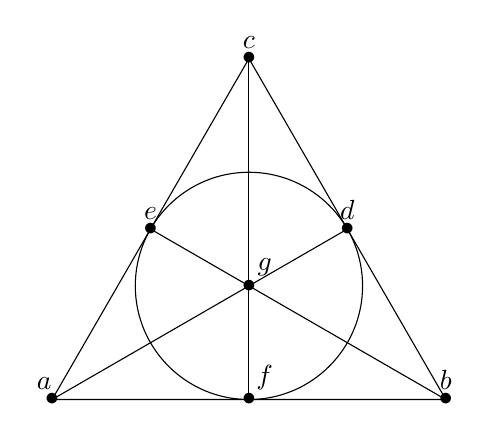
\begin{tikzpicture}[scale = .5]
\node[coordinate, label={[shift={(-.1,0)}]$a$}] (a) at (-5, -4.33) {$\bullet$};
\node[coordinate, label={[shift={(0,0)}]$b$}] (b) at (5, -4.33) {$\bullet$};
\node[coordinate, label={[shift={(0,0)}]$c$}] (c) at (0, 4.33) {$\bullet$};
\node[coordinate, label={[shift={(0,0)}]$d$}] (d) at (2.5, 0) {$\bullet$};
\node[coordinate, label={[shift={(0,0)}]$e$}] (e) at (-2.5, 0) {$\bullet$};
\node[coordinate, label={[shift={(.2,0)}]$f$}] (f) at (0, -4.33) {$\bullet$};
\node[coordinate, label={[shift={(.2,0)}]$g$}] (g) at (0, -1.44325)
{$\bullet$};
\foreach \x in {a, b, c, d, e, f, g}
    \draw (\x) node {$\bullet$}; 

\draw (a) -- (b)--(c)--(a);
\draw (a) -- (d);
\draw (b) -- (e);
\draw (c) -- (f);
\draw (g) circle (2.8865);

\end{tikzpicture}
\end{center}

 Given this setup, the bases sets of the Fano matroid are specifically the triples that do not lie on any given line or circle. Namely, the sets $\{f, g, d\}$, $\{a,b, c\}$, $\{d, b, f\}$ etc. The circuits of rank 2 are exactly the cyclic flats. Circuits of rank 3 are the sets of 4 elements with any line or circle containing exactly two elements. E.g. $\{c, e, g, d\}$ is a cicuit of rank $3$, but $\{f, g, a, c\}$ is not because $\{f, g, c\}$ is a set of $3$ colinear points. 
\end{eg}

\subsection{Matroids as hypergraphs \label{sec:matroidhypergraph}}

In this section, we give a hypergraphical condition for when  set $\sC$, defines the circuits of a matroid. Note that this is different from the notion of a hypergraphic matroid ala Lorea \cite{1975_paper}. \hlfix{This is the ??? construction}{must exist in the literature. figure out where.}

First, recall that a hypergraph is a pair $G = (V, E)$ where each edge $E$ corresponds to a non-empty subset of $V$ (as opposed to a pair of elements of $V$). We denote the vertices of the hyper edge $e$ as $V(e)$. In this manner, for any subgraph $H \subseteq G$, we denote by $|H|$ the number of edges in the subgraph and by $V(H) = \cup_{h \in H} V(h)$ the vertices contain in the subgraph. As with regular graphs, one may speak of connected components of the hypergaph.  In the following, we need a definition of a minimal hyperedge chain.

\begin{dfn} \label{dfn:minhypergraphchain}
    A hyperdge chain in the hypergraph $G$ is an ordered list of hyper edges $\{e_1, \ldots, e_k\}$ such that  $V(e_i) \cap V(e_{i+1}) \neq \emptyset$. Such a hyperedge chain is minimal if  
    \begin{itemize}
    \item Removing any internal edge $e_i$, $i \not \in \{1, k\}$, results in two disconnected components,  $\{e_1, \ldots, e_{i-1}\}$ and $\{e_{i+1}, \ldots, e_k\}$
    \item Any other chain between edges $e_1$ and $e_k$ has more edges.
    \end{itemize}
\end{dfn}

Similar to graphs, one can define hyper triangles on graphs.

\begin{dfn} \label{dfn:hypertriangle} \sanote{better? is this a known type of triangle?}
    A hyper triangle is a triple of hyper edges $\{e_1, e_2, e_3\}$ that pairwise intersect, $e_i \cap e_j \neq \emptyset$ and that have no common intersection: $e_1 \cap e_2 \cap e_3 = \emptyset$. We further insist that the triangles lack an inclusion of intersections, $e_i \cap e_j \not \subseteq e_i \cap e_k$, and that there is no edge containment, $e_i \not \subseteq e_j$. 
\end{dfn}

This is the natural generalization of edge chains on (multi) graphs. 

\begin{rmk}\label{rmk:onintersections}
Note that the definition of minimal hyperedge chains implies that if $V(e_i) \cap V(e_{i+1}) \subseteq V(e_i) \cap V(e_{i-1}) $ for a sequence of hyperedges $\{e_1, \ldots, e_k\}$ then the sequence is not minimal. Namely, removing $e_i$ gives $\{e_1, \ldots, e_{i-1}, e_i, \ldots, e_k\}$ which remains connected.
\end{rmk}

We are now ready to give a hypergraphical representation of the circuit sets of matroids. First we recall the strong circuit condition.

\begin{dfn}
    The set $\sC$ is the circuit set of a matroid if:
    \begin{enumerate}
    \item $\emptyset \not \in \sC$
    \item If $C_1, C_2 \in \sC$ then $C_1 \not \subseteq C_2$.
    \item If $x \in C_1 \cap C_2$, let $y \in C_1 \setminus C_2$. Then there is a $C_3 \in \sC$ such that $y \in C_3$ and $C_3 \subseteq (C_1 \cup C_2) \setminus x$.
    \end{enumerate}
\end{dfn}

\begin{comment}show an that the third circuit, whose existence is demanded by the circuit condition, \eqref{eq:circuitcondition},, must contain the symmetric difference of the two initial circuits.

\begin{lem}\label{res:symdiffcontained}
Let $M = (V, \sC)$. Then, for $x \in C_1 \cap C_2$ and $C_3 \subseteq C_1 \cup C_2 \setminus x$, $C_3$ contains the symmetric difference of $C_1$ and $C_2$: $C_3 \supseteq (C_1 \cup C_2) \setminus (C_1 \cap C_2)$.
\end{lem} \sanote{this is not correct. See strong circuit cond}
\begin{proof}
Suppose that $C_3 \supseteq (C_1 \cup C_2) \setminus (C_1 \cap C_2)$ does not hold. Since $C_3 \subseteq C_1 \cup C_2 \setminus x$, this implies that $C_3 \subsetneq (C_1 \cup C_2) \setminus (C_1 \cap C_2)$. I.e. there is an element $a \in C_2\setminus C_1$ such that $a \not \in C_3$. 

Since $C_3 \not \subseteq C_2$,  $|(C_1 \setminus C_2)\cap C_3| = n_3$ with $y_3 \in C_1 \cap C_3$ Note that $C_2 \not \subseteq C_1 \cap C_3 \setminus y_3$. Therefore, by the circuit condition, \eqref{eq:circuitcondition}, there is a $C_4 \subseteq C_3 \cap C_2 \setminus y_3$. If $n_3 = 1$ then $C_4 \subsetneq C_2$, which is a contradiction.

If $n >1$, $|(C_1 \setminus C_2)\cap C_4|  = n_4 < n_3$. Let $y_4 \in C_3 \cap C_4$, and $C_5 \subseteq C_3 \cap C_4 \setminus y_4$. If $m = i$, then $C_5 \subsetneq C_2$, which is a contradiction. Otherwise, continue applying the circuit condition, \eqref{eq:circuitcondition}, to get $C_{i+1} \subseteq C_3 \cup C_i \setminus y_i$ with $|(C_1 \setminus C_2)\cap C_i|  = n_{i+1} < n_i$. This will yeild $n_k = 1$ for some $k$, forcing $C_{k+1} \subsetneq C_2$ which is a contradiction. 
\end{proof} \end{comment}


This gives rise to an important corrollary that we use in defining the hypergraph structure.

\begin{cor}\label{res:2-complete}
If $M = (V, \sC)$, and $C_1, C_2 \in \sC$ are circuit with non-empty intersection, $C_1 \cap C_2 \neq \emptyset$, then for every $a \in C_1$ and $b \in C_2$, both $a$ and $b$ are contained in a circuit in $\sC$.
\end{cor}
\begin{proof}
Suppose not. That is, $x, a \in C_1$ and $x, b \in C_2$ \esnote{introduce x seperately}, but any $C \in \sC$ containing $b$ does not contain $a$ and any $D \in \sC$ containing $a$ does not contain $b$. Let $C, D \subseteq C_1 \cap C_2 \setminus x$. \esnote{C and D don't get used.} The existence of such sets is guaranteed by the strong circuit condition.

Let $C_3 \subsetneq C_1 \cup C_2 \setminus x$ contain $a$ but not $b$. There is an element $y_3 \in C_3 \cap C_2$, and $y_3 \neq b$. Let $C_4 \subseteq C_2 \cup C_3 \setminus y_3$. By the strong circuit condition, we may choose $C_4$ to contain $b$, since $b \in C_2 \setminus C_3$. Note that $C_4$ contains an element in $C_3 \cap C_1$ (otherwise $C_4 \subseteq C_2$, which is not allowed). Let $y_4 \in C_4 \cap C_1 \cap C_3$. Furthermore, since $b \in C_4$, $a\not \in C_4 \cap C_1$. Therefore, we have that $|C_4\cap C_1| \leq |(C_3 \cap C_1) \setminus \{a\}| $. 

Next we find a $C_5 \subseteq C_4 \cup C_3 \setminus y_4$. Therefore, $a, y_4 \not \in C_5 \cap C_4 \cap C_1$. However, this intersection is not empty (otherwise $C_5 \subseteq C_2$, which is not allowed \esnote{But since $C_4$ is a subset with an intersection of $C_2$ this should aways be true}). Let $y_4 \in C_5 \cap C_1 \cap C_4$. Therefore, we have that $|C_5\cap C_1| \leq |(C_3 \cap C_1) \setminus \{a, y_4\}| $.

Continuing, in this manner, for any $i > 4$, one can always find a $C_i \subset C_{i-1} \cup C_{i-2} \setminus y_{i-1}$ containing $b$ with $a, y_4, \ldots, y_{i-1} \in C_i \cap C_{i-1} \cap C_1$ and $|C_i\cap C_1| \leq |(C_3 \cap C_1) \setminus \{a, y_4, \ldots, y_{i-1}\}|$. By finiteness of the groundset, this is impossible.
\end{proof}

\begin{center}
		\scalebox{1}{
			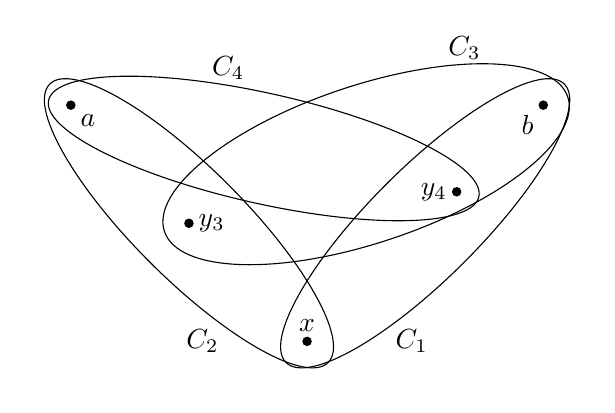
\begin{tikzpicture}[scale=1]
				
				\filldraw (0,0) circle[radius=1.5pt];
				\node[above] at (0,0) {$x$};
				\filldraw (-3,3) circle[radius=1.5pt];
				\node[below right] at (-3,3) {$a$};
				\filldraw (3,3) circle[radius=1.5pt];
				\node[below left] at (3,3) {$b$};
				\filldraw (-1.5,1.5) circle[radius=1.5pt];
				\node[right] at (-1.5,1.5) {$y_{3}$};
				\filldraw (1.9,1.9) circle[radius=1.5pt];
				\node[left] at (1.9,1.9) {$y_{4}$};
				\draw[rotate around={-45:(-1.5,1.5)}] (-1.5,1.5) ellipse (2.5cm and 0.7cm);
				\draw[rotate around={45:(1.5,1.5)}] (1.5,1.5) ellipse (2.5cm and 0.7cm);
				\draw[rotate around={18.43:(0.75,2.25)}] (0.75,2.25) ellipse (2.7cm and 1cm);
				\draw[rotate around={-12.65:(-0.55,2.45)}] (-0.55,2.45) ellipse (2.8cm and 0.7cm);
				
				\node[right] at (1,0) {$C_{1}$};
				\node[left] at (-1,0) {$C_{2}$};
				\node[above] at (2,3.45) {$C_{3}$};
				\node[above] at (-1,3.2) {$C_{4}$};
			\end{tikzpicture}
		}
\end{center}

We are now ready to prove that matroids give rise to hypergraphs with 2-complete connected components. Recall that a hypergraph is 2 complete if every pair of vertices is contained in a hyperedge.

\begin{lem}\label{res:matroidthenhypergraph}
    Let $M = (V, \sC)$ be a matroid. Then $G = (V, \sC)$ is a  hypergraph where every connected component is $2$-complete.
\end{lem}
\begin{proof} \sanote{fix this proof}
    Suppose that $H$ is a connected component of $G$. Let $a \in C_0$ and $b \in C_{2n+1}$ \esnote{where is $n$ coming from?} for $C_0, C_{2n+1} \in H$. Since $H$ is a connected component, there is a sequence of overlapping edges $\{C_0, C_2, \ldots C_{2n}\}$ such that $x_i \in C_{2i}\cap C_{2(i-1)}$ \esnote{What are the $x_i$'s} and $x_{n+1} \in C_{2n} \cap C_{2n+1}$ \esnote{for what values of $i$?}. Consider the shortest chain where $a$ is in the first hyperedge and $b$ in the last. By Remark \ref{rmk:onintersections}, there is an $x_i \in C_{2i}\cap C_{2(i-1)}$ that is not in the previous intersection: $x \not \in C_{2(i-1)}\cap C_{2(i-2)}$.
    
    Since $M$ is a matroid, and hyperedges correspond to circuits, we know that there is an edge $C_1 \subseteq C_0 \cup C_2 \setminus x_1$. Note that $a \in C_0 \setminus C_2$ (otherwise one could set $C_2$ to $C_0$ and shorten the chain). Similarly, $x_2 \in C_2 \setminus C_0$. By Corollary \ref{res:2-complete}, $a, x_2 \in C_1$. Similarly, there is an edge $C_{2i-1} \subseteq C_{2i-3} \cup C_{2i} \setminus x_i$ with $a, x_{i} \in C_{2i-1}$. Thus, $a \in C_{2n-1}$ and $b \in C_{2n+1}$ with $x_{n+1} \in C_{2n} \cap C_{2n+1}$. The circuit condition, \eqref{eq:circuitcondition}, and Corollary \ref{res:2-complete} implies that there is a hyperedge $C \subseteq C_{2n} \cup C_{2n+1} \setminus x_{n_1}$ that contains both $a$ and $b$. 
\end{proof}

Not all hypergraphs with 2-complete connected components give rise to matroids. One needs to explicitly specify the conditions on the hyperedges make them interpretable as circuts. 

\begin{lem}\label{res:somehypergraphsmatroids} \sanote{Everett: are the two conditions below hyper graph theoretic}
    Let $G = (V, E)$ be a hypergraph. For $e \in E$, write $V(e) \subseteq V$ to indicate the vertices of $e$. Then $G$ defines a matroid if and only if it satisfies the following conditions:\begin{enumerate}
        \item For every distinct $e, f \in E$, the the vertices of $V(e) \not \subset V(f)$.
        \item If $x \in V$ is a vertex shared by $e$ and $f$, $x \in V(e) \cap V(f)$, then there is an edge $g$ with $V(g) \subseteq V(e) \cup V(f) \setminus x$
    \end{enumerate}
\end{lem}

\begin{proof}
    These are exactly the conditions necessary to interpret the collection of sets $\{ V(e) | e \in E\} $ as the circuit set of a matroid.
\end{proof}


\subsection{Matroid completion of hypergraphs}

In this section, we give an algorithm to find a set of matroids contained in a given independence system. 

\begin{lem}\label{res:circuitinclusion}
    Given two independence systems $\sI$ and $\sI'$,let $\sC$ and $\sC'$ be the corresponding sets of circuits. Then the inclusion $\sI \subseteq \sI'$ holds if and only if for every $C' \in \sC'$, there is a $C \in \sC$ such that $C \subseteq C'$.
\end{lem}
\begin{proof}
    Since $\sI \subseteq \sI'$ the dependent sets of $\sI$ contain the dependent sets of $\sI'$: $\sI^{'c} \subsetneq \sI^c$. Therefore, if $C'$ is minimal in $\sI^{'c}$, then $C' \in \sI^c$, but not necessarily minimal. Therefore, there is a $C \in \sC$ such that $C \subseteq C'$.

    Conversely, if for every $C' \in \sC'$, there is a $C \in \sC$ such that $C \subseteq C'$, then, the set of sets containing elements of $\sC$ is larger than the set of sets containing elements of $\sC'$. In other words, $\sI^c \supseteq \sI^{'c}$, or $\sI \subseteq \sI'$. 
\end{proof}

Let $\sC$ be the minimally dependent sets of some independence system, not necessarily a matroid. We write $G_\sC = (V, \sC)$ to be the associated hypergraph. 

\begin{dfn} \label{dfn:triples}
    For $\sC$ a minimally dependent sets of some independence system, the set $T(\sC)$ is the set of triples, $(x, C_1, C_2)$ such that $C_1, C_2 \in \sC$ and $x \in C_1 \cap C_2$: \bas T(\sC) = \{  (x, C_1, C_2) | C_1, C_2 \in \sC; \;  x \in C_1 \cap C_2\} \;.\eas Define $C_T = C_1 \cup C_2 \setminus x$.
\end{dfn}

We claim the following algorithm gives rise to a matroid $M = (V, \sS)$, where $\sS$ is the circuit set of $M$ and is contained in the independence system of $\sC: \sI(\sS) \subseteq \sI(\sC)$.

\begin{alg} \label{alg:largestmatroid}
    To initialize, let $\sS = \sC_0 = \sC$, and $\cT = T(\sS)$. 

    If $\cT = \emptyset$, then return $\xC$.
    
    If $|\cT| >0$ select $T \in \cT$. \esnote{What is $\cT$ is empty? (It should be spelt out that the algorithm stops)}
    \begin{enumerate}
        \item If $\exists C \in \sS$ such that $C \subseteq C_T$,
        \begin{enumerate}
            \item Set $\cT := \cT \setminus T$, 
            \item Leave $\sS$ unchanged 
            \item Restart the algorithm with these new values.
        \end{enumerate}
        \item If $\not \exists C \in \sC$ such that $C \subseteq C_T$
        \begin{enumerate}
            \item Define $\cC_T = \{C \in \sS | C_T \subsetneq C\}$ to be the set of elements of $\sC$ properly containing $C_T$
            \item Set $\sC_{i+1} := (\sS \cup C_T) \setminus \cC_T$
            \item Set $\cT := T(\sC_{i+1})$.
            \item Set $\sS := \sC_{i+1}$.
            \item Restart the algorithm with these new values. 
        \end{enumerate}
    \end{enumerate}
\end{alg}

\begin{rmk} \label{rmk:algoexplained}Note that if there is a $C \in \sC$ such that $C_T \subseteq C$ at some stage, then the circuit condition, \eqref{eq:circuitcondition}, is met for the triple $T$. Therefore, the algorithm does not change the set $\sS$. If such a $C$ does not exists, then $C_T$ is added to the set (in order to ensure that the circuit condition holds. In order to preserve that $\sS$ is a minimally dependent set of some independence system (i.e. property \eqref{eqn:minmaxset}), the algorithm removes and preexisting $C \in \sS$ that contains the newly added $C_T$. Adding and shrinking sets in $\sS$ changes the class of associated triples. Therefore, the algorithm needs to be started afresh with a new set of triples every time $\sS$ is changed. \end{rmk}

For the rest of this section, we show that the set $\sS$ resulting from algorithm \ref{alg:largestmatroid}, when starting with $\sC$, gives rise to a largest matroid whose independence system is contained in $\sI(\sC)$. 

\begin{rmk}\label{rmk:placementmonotonic}
    Note that if $C_T$ is a set added to $\sS$ at some step in Algorithm \ref{alg:largestmatroid}, with $T = (x, C_1, C_2)$, then $|C_T| \geq |C_1|$ and $|C_T| \geq |C_2|$.
\end{rmk}

\begin{lem} \label{res:algoterminates}
    Algorithm \ref{alg:largestmatroid} terminates in a finite number of steps. 
\end{lem}
\begin{proof}
    Algorithm \ref{alg:largestmatroid} introduces new sets to the collection $\sC$. By Remark \ref{rmk:placementmonotonic}, the set place, $C_T$ is at least as big (in terms of number of elements) as the other two sets in the hyper triangle. Therefore, by finiteness of the set of sets $2^V$, and the monotonicity of the size of sets pladed by the algorithm, the algorithm terminates.
\end{proof}

Next we show that if a set in the final out put is not an element of the input, then it is part of a hyper triangle in $G_\sS$.

\begin{lem} \label{res:placedsetsCT}
    If $S \in \sS$, then it is either in $\sC$ or it is of the form $C_T$ for some $T \in T(\sS)$.
\end{lem}
\begin{proof}
Note that at some stage in the algorithm, $S = C_T$ for some $T \in T(\sC_{i})$. Write $T = (x, S_1, S_2)$. If at some later stage, $j > i$, $S_1 \not \in \sC_j$, then some subset is, $T_1 \in \sC_j$ where $T_1 \subsetneq S_1$. If $T' = (x, S_1, T_2) \in T(\sC_j)$ then $S \supsetneq C_{T'}$, and therefore $S \not in \sS$. If $T' \not \in T(\sC_{j})$ then either $S_1 \subsetneq S$ or $C_{(y, S_1, T_2} \subsetneq S$ for some $y \in S_1 \cap T_2$. In either case, $S$ is removed at this stage. Therefore, if $S = C_T \in \sS$, and first introduced at step $\sC_i$, there is no later stage when the other ends of the triangle are contracted.
\end{proof}

Note that this this algorithm does not require that every vertex in the ground set is involved in the set of minimal dependent sets: $V \supseteq \cup_{C \in \sC} C$. Similarly,  the vertices involved in the set $\sS$ are contained in the vertices involved in $\sC$: $\cup_{S \in \sS} S \supseteq \cup_{C \in \sC} C$. 



\begin{lem}\label{res:algogivesminimal}
    If Algorithm \ref{alg:largestmatroid} outputs the set of sets $\sS$, then $\sS$ is the minimal dependent sets for an independence system.
\end{lem}
\begin{proof}
    Note, as in the proof of Lemma \ref{res:algoterminates}, Algorithm \ref{alg:largestmatroid} only adds sets and removes sets. It only adds a set if there is not another set in existence at that stage that would be a subset of the set to be added. 

    Similarly, after a set is added, as explained in Remark \ref{rmk:algoexplained}, the algorithm check for any existing sets that contain the added set, and removes those.

    Thus, at every intermediary stage, the intermediate results of the algorithm satisfies property \eqref{eqn:minmaxset}. Therefore, so does the output. In other words, $\sS$ can be interpreted as the minimal dependent sets of an independence system.
\end{proof}

Next we show that Algorithm \ref{alg:largestmatroid} results in an inclusion of independence systems.

\begin{lem}\label{ref:algogivesinclusion}
    If Algorithm \ref{alg:largestmatroid} outputs $\sS$ with the input of $\sC$ the the independence system $\sI(\sS) \subset \sI(\sC)$.
\end{lem}
\begin{proof}
    By Lemma \ref{res:algogivesminimal}, $\sS$ can be interpreted as a minimal dependent set of some independence structure. Therefore, $\sI(\sS)$ is a well defined object. 

    Note that, by construction, if $C \in \sC \setminus \sS$, there is an $S \in \sS$ such that $S \subsetneq C$.
    By Lemma \ref{res:circuitinclusion}, this implies that $\sI(\sS) \subset \sI(\sC)$. 
\end{proof}

Next we show that Algorithm \ref{alg:largestmatroid} results in a matroid.
\begin{lem} \label{res:algogivesmatroid} If Algorithm \ref{alg:largestmatroid} outputs $\sS$, then $(V, \sS)$ defines the circuit set of a matroid.
\end{lem}
\begin{proof}
    Lemma \ref{res:algogivesminimal} shows that $\sS$ can be interpreted as the set  of minimal dependent sets of some independence structure. Therefore, it only remains to check that it satisfies the circuit condition, \eqref{eq:circuitcondition}.

    In order to assure this, for the final output, $\sS$, the algorithm checks that for every relevant triple, $T = (x, C_1, C_2)$ with $C_1, C_2 \in \sS$, and $x \in C_1 \cap C_2$, there is another $C \in \sS$ such that $C \subseteq C_T$. In other words, that \eqref{eq:circuitcondition} is satisfied.
    \end{proof}

It is worth noting that Algorithm \ref{alg:largestmatroid} does not result in a unique set $\sS$. Specifically, the outputted set $\sS$ depends on the order in which one selects triples $T$ from the set $T(\sS)$. 

\begin{eg} \label{eg:ordermatters}

WRITE UP EXAMPLE HERE!
    
\end{eg}

Before proving that $\sS$ defines the largest matroid contained in $\sC$, we prove an useful observation about the structure of the hypergraphs $G_\sC = (V, \sC)$ and $G_\sS = (V, \sS)$.

\begin{lem}\label{res:orginaledgeineachcc}
    Let $H \subset G_\sS$ be a connected component. There is some $C \in \sC$ such that $C \in H$.
\end{lem}
\begin{proof}
    Define $\cC  = \{C \in \sC | \exists S \subseteq C, \; S\in  H\}$. Chose $C \in \cC$ such that there is no $C' \in \cC$ such that $|C'| < |C|$.

    If $C \not \in H$, there is some $S \subsetneq C$ in $H$. Specifically, $|S| < |C|$. Since $S \not \in \sC$, $S = C_T$ for some $T = (x, S_1, S_2) \in T(\sS)$. Therefore, by Remark \ref{rmk:placementmonotonic} $|S_1|, |S_2| \leq |S| < |C|$. Working backwards through the algorithm, one eventually finds a $C' \in \sC$ that is part of a hyper triangle that defines one of the hyper edges needed to form a triangle involving $S_1$ or $S_2$. By Remark \ref{rmk:placementmonotonic}, $|C'| < |C|$, which is a contradiction.
\end{proof}


\begin{lem} \label{res:orginaledgesubsetineachcc}
    Let $H \subseteq G_\sS$ be a connected component. If $|H| = 1$, then $S \in H$ is also in $\sC$. If $|H| >1$ then there is an intersecting pair of sets in $H$, that are also subsets of sets in $\sC$: $S_1, S_2 \in H$ such that $S_1 \cap S_2 \neq \emptyset$, $S_1 \subseteq C_1, S_2\subseteq C_2$ for $C_1, C_2\in \sC$.
\end{lem}
\begin{proof}
    First note that if $S \in \sS$, then $S \in \sC$ or $S = C_T$ for some $T \in T(\sS)$. Therefore, if $H$ is a connected component with just one element, $S$, $S$ cannot be of the form $C_T$. Therefore $S \in \sC$.

    Now suppose $|H| >1$. By the circuit condition, \eqref{eq:circuitcondition}, one cannot have $|H| = 2$. Therefore,  $|H| \geq 3$. Suppose there is not an $T = (x, S_1, S_2) \in T(H)$ such that $S_1 \subseteq C_1, S_2\subseteq C_2$ for $C_1, C_2\in \sC$. Specifically, suppose $S_2$ is not contained in any $C \in \sC$. We proceed by induction and contradiction. 
    
    At some earlier, intermediate stage of Algorithm \ref{alg:largestmatroid}, there is a $T_2 = (x_2, S_3, S_4)$ in $T(\sS)$ where $S_2  \supseteq C_{T_2}$. Furthermore, the sets $S_3, S_4$ appeared earlier in the algorithm than $S_2$. We may have that $S_3 = S_1$, but $S_4$ is  not in any $C \in \sC$. Suppose for all $k$, the set $S_{2k}$ is not in any $C \in \sC$. Then there must be a $T_{2k} = (x_{2k}, S_{2k+1}, S_{2(k+2)})$ where $S_{2k} \supseteq C_{T_{2k}}$ and $S_{2(k+2)}$ existed at an earlier stage of the algorithm but $S_{2(k+2)}$ not in any $C \in \sC$. However, by Lemma \ref{res:algoterminates}, Algorithm \ref{alg:largestmatroid} terminates in finite time. Therefore, for some $k$, $S_{2k-1} \subseteq C$ , $S_{2k} \subseteq C'$ with  $C, C'\in \sC$ and $x_{2k} \in S_{2k-1} \cap S_{2k} $. 

\end{proof}

Finally, we show that for any $\sS$ that is the output of Algorithm \ref{alg:largestmatroid}, the set $\sI(\sS)$ is the largest matroid contained in $\sI(\sC)$.  

\begin{thm}
    Let $\sS$ be a set of minimal dependent sets outputted by Algorithm \ref{alg:largestmatroid} for the input set $\sC$. Then $M = (V, \sS)$ is a maximal matroid contained in the independence data $\sI(\sC)$ under containment of indepence systems. 
\end{thm}
\begin{proof}
    If $\sC$ is the empty set, then $\sS$ is the empty set. We prove the theorem for $\sC \neq \emptyset$.
    
    Suppose that there is another set of circuits of a matroid, $\sR$ such that $\sI(\sS) \subsetneq \sI(\sR) \subsetneq \sI(\sC)$. 

    Note that by construction, if $S \in \sS$, then either $S \in \sC$ or $S = C_T$ for some $T = (x, C_1, C_2)$ with $C_1, C_2 \in \sS$ and $s \in C_1 \cap C_2$.

    There are two cases to consider: when every set in $\sR$ is contained in $\sS$, and when there is a set $R \in \sR$ such that there is an $S \in \sS$ such that $S \subsetneq R$.

    In the first case, since $\sC$ is not empty, Lemma \ref{res:circuitinclusion} implies that $\sR$ is not empty. Since, $\sI(\sS) \neq \sI(\sR)$, there is a proper, non-empty subset $\cS \subsetneq \sS$ such that $\sR = \sS \setminus \cS$. There are two subcases, when $\cS$ does and does not form a connected component of $G_\sS$. 
    \begin{enumerate}
        \item If the edges $\sC$ do not form a connected component of $G_\sS$, then let $H$ be a connected component of $G_\sS$ such that has a proper, non-empty subset of hyperedges in $\sC$: $H \setminus \sC \neq \emptyset$ and $H \cap \sC \neq \emptyset$. Since $\sS$ defines a matroid, the circuit condition, \eqref{eq:circuitcondition}, there is some $S \in \cS$ is of the form $S \subseteq C_T$ for some $T \in T(H\setminus \cS)$, $T = (x, R_1, R_2)$.  Write $A  = (R_1 \cup R_2) \setminus (R_1 \cap R_2)$. Let $y \in S$ be an element of $A$. Since $\sR$ is also a matroid, there is an $R \in H\setminus \cS$ that is also a subset of the same $C_T$. Write $T' = (y, S, R)$ Any $Q \subseteq C_{T'}$ has fewer elements in $A$ than $R$. Following the agruments in Lemma \ref{res:2-complete}, we see that repeated application of the circuit condition to sets contained in $C_T$ results in a set in $\sR$ that is a subset of either $R_1$ or $R_2$, which is a contradiction.
        \item If $\cS$ is a connected component of $G_\sS$, by Lemma \ref{res:orginaledgeineachcc}, there is a $S \in \cS$ such that $S \in \sC$. By construction, $S \not \in \sR$. Therefore, by \ref{res:circuitinclusion}, $\sI(\sR) \not \subseteq \sI(\sC)$. \end{enumerate}
    
    In the second case, there is some $S \in \sS$ and $R \in \sR$ such that $S \subseteq R$. Note that if $S \in \sS$, $S \in \sC$ or $S = C_T$ for some $T \in T(\sS)$. 
    \begin{enumerate} 
    \item If $S \in \sC$ and $S \in R$ then by \eqref{eqn:minmaxset}, there is no $R' \in \sR$ such that $R' \subseteq S$. In other words, $\sI(\sR) \not \subseteq \sI(\sC)$. 
    \item If $S = C_T$ for some $T = (x, S_1, S_2) \in T(\sS)$, consider $a \in R \setminus S$. Since $\sR$ defines a matroid, $R \subseteq C_{T'}$ for $T' = (x, R_1, R_2) \in T(\sR)$ and that $a$ is in at least one of $R_1$ or $R_2$, assume $R_1$. We claim that at least one of $C_1$ or $C_2$ (and its subsets) are not in $\sR$. If both $C_1, C_2 \in \sR$, then, by the circuit condition, \eqref{eq:circuitcondition}, there is a  $Q \subseteq C_T$ with $Q \in \sR$. But $Q \subseteq R$ which contradicts the minimality condition, \eqref{eqn:minmaxset}. Similarly for any subset of $S_1$ or $S_2$. Therefore, assume $S_1$ and its subsets are  not in $\sR$. Similarly, for all hyper triangles in $G_\sS$ involving $C_1$, both of the other two hyper edges or their subsets are not in $\sR$.
    
    Let $H$ be the connected component of $G_\sS$ containing $S$.  By Lemma \ref{res:orginaledgeineachcc}, there is a $C \in \sC$ such that $C \in H$. Since $H$ is a connected component of $G_\sS$, there is a path of hyperedges connecting $S$ to $S_1$, $\{C = e_0, e_1, \ldots, e_k = S_1 \}$. Since $H$ is $2$ complete, each $e_i$ is involved in a hyper triangle, where one of the other edges is in a hyper triangle with $e_{i-1}$. Therefore, by the above argument, $C \not in \sR$. Therefore, by Lemma \ref{res:circuitinclusion}, $\sI(\sR) \not \subseteq \sI(\sC)$. 
    \end{enumerate}
Having shown that all possible cases lead to a contradiction of the existence of  an $\sR$ such that $\sI(\sS) \subsetneq \sI(\sR) \subsetneq \sI(\sC)$, Algorithm \ref{alg:largestmatroid} must result is a maximal matroid with independence set in $\sI(\sC)$.
\end{proof}

\section{Positroids}
For the remainder of this paper, we are interested in studying a particular class of matroids, positroids. In particular, we are interested in identifying the largest positroids contained in a matroid. Note that as with a matroid, a positroid is contained in a matroid (or another positroid) if and only if there is containment of the associated independence systems. 

Unlike a matroid, the ground set of a positroid is a cyclically ordered set. We denote by $[n]$ the cyclically ordered set $\{1, \ldots, n\}$. We denote by $<_i$ the linear ordering on $[n]$ starting at the element $i$. That is $i <_i (i+1) \ldots <_i n <_i \ldots 1 \ldots <_i (i-1)$. Therefore, for the rest of this paper, we consider matroids defined on a cyclically ordered set. 
 
\begin{dfn}\label{dfn:positroid}
A positroid is a representable matroid over the base field $k$ over the ground set $[n]$, where every maximal minor of every representing matrix is non-negative. 
\end{dfn}

There are several different combinatorial tools that enumerate the positroids, the equivalence of which is defined in \cite{Postnikov}. In this section, we discuss two of them, Grassmann necklaces and Le diagrams.

\begin{dfn} \label{dfn:GN} A Grassmann necklace is a cyclically ordered set of $n$ elements, each of which is a set of $k$ elements, $\cI = \{I_1, \ldots , I_n\}$ such that, if $i\in I_i$, there is some other element $j \neq i$ such that $I_{i+1} = \left(I_i \setminus i\right) \cup j$. If $i \not \in I_i$ then $I_i = I_{i+1}$.
\end{dfn}

\begin{dfn} \label{dfn:Le}
    A Le diagram (of type $(k, n)$) is a Young tableau placed in side a $k \times (n-k)$ box with $0$'s and $+$'s in the entries, and the eastern and southern edges labeled by the entries $\{1, \ldots, n\}$ ordered from the north east most edge to the south west most. Furthermore, each $0$ in the diagram either has only $0$'s north of it or has only $0$'s west of it.
\end{dfn}

Let $M = ([n], \sB)$ be a positroid defined on the ground set $[n]$ with rank $\rk(M) = k$. Then order the elements $I_i$ in the associated Grassmann necklace given by the lexicographically minimal elements of $\sB$ in the $<_i$ order. Call this $\cI_\sB$.

Furthermore, each Grassmann necklace $\cI$ defines a bases set, $\sB_\cI$. First we define the Gale order, which is a partial order on subsets of a cyclically ordered sets. 

\begin{dfn} \label{dfn:Gale} For $A, B \subseteq [n]$ with $|A| = |B|$, in the $<_i$ linear order write $A = A^{(1)} <_i A^{(2)} <_i \ldots <_i A^{(k)}$. Then $A \preceq_i B$ in the Gale order  if and only if $A^{(i)} \leq_i B^{(i)}$ for all $i$. \end{dfn}

A Grassmann Necklace $\cI$ defines a basis set \ba \sB_\cI = \{ B | I_i \preceq_i B \; \forall i \in [n]\} \;. \label{eq:I_B} \ea 
The matroid $(\sB_\cI, [n])$ is a positroid. In fact, given a matroid $M = (\sB, [n])$, the independence system associated to $\sB_{\cI_\sB}$ is the smallest positroid containing $\sB$. 
Furthermore, the two independence structures are equal if and only if $\sB$ is the basis set for a positroid \cite{Postnikov}.

A Le diagram defines the basis set of a positroid as shown in Section ??? of \cite{Postnikov}. Similarly, the basis set of a positroid defines a Le diagram by placing $+$'s in the appropriate boxes. This process is describes in \cite{Postnikov}, and not repeated here. There are algorithms to read off the Grassmann necklace of  a positroid from the Le diagram \cite{Oh}, and to find the Le diagram associated to a Le diagram \cite{GNtoLe}. 

Finally, it is work mentioning a third combinatorial tool in one to one correspondence to Le diagrams, namely word, sub-word pairs in the alphabet of Coxeter generators of the symmetric group $S_n$ \cite{Juggling}. These word, subword pairs are useful for understanding a geometry associated to postroids.

Note that for a positroid of rank $k$ with ground set $[n]$ defined over $\R$, the matrices representing it are elements of $\Gr(k,n)$, i.e. the part of $\Grall(k,n)$ with non-negative Pl\"{u}cker coordinates. These point define a CW complex over $\Gr(k,n)$. For $M$ a positroid, we denote by $\Sigma(M) \subset \Gr(k,n)$ the associated positroid cell\cite{GrBall, Postnikov}.  The boundary of each positroid cell is the union of lower dimensional positroid cells. 

The dimension of a positroid cell can be determined from the Le diagram, by counting the number of $+$'s. There is an algorithm, \cite{notes}, to calculate the boundaries of a positroid cell from the word, subword pairs. However, one must pass to the Le diagram to calculate the codimensions of said boundaries.  One application of the algorithm in this paper, is to identify codimension one boundaries of a given positroid.

\subsection{Positroids as hypergraphs \label{sec:positroidhypergraph}} 

As above, let $M = ([n], \sC)$ be a matroid defined on the cyclic set $[n]$, with $\sC$ its circuit set. Write $G_M = ([n], \sC)$ as the hyper graph on $n$ with hyper edges corresponding to the elements of $\cC$. From Lemma \ref{res:matroidthenhypergraph}, we know that every connected component is two complete. From Lemma \ref{res:somehypergraphsmatroids} we know that the hyper edges of $G_M$ satisfy the circuit condition. 

In this section, we give a criterion for when a graph of the form $G_M$ defines a positroid. First we define crossing sets.

\begin{dfn} \label{dfn:crossingsets}
    For any subset $A \subset [n]$, we can partition $A$ into disjoint cyclically ordered connected components, $A = A_1 \sqcup \ldots \sqcup A_r$. Similarly, the complement can be written in terms of cyclically ordered connected components: $A^c = A_1^c \sqcup \ldots \sqcup A_r^c$. Two sets $A$ and $B$ are crossing if multiple components of the cyclic intervals of $A^c$ contain elements of $b$. I.e. there $b_i, b_j \in B$ such that $b_i \in A^c_i$ and $b_j \in A^c_j$. 
\end{dfn}

Note that if $A$ can be decomposed into cyclically ordered connected components, so can its complement: $A^c = A^c_1 \sqcup \ldots \sqcup A^c_r$. An equivalent definition to Definition \ref{dfn:crossingsets} is that $A$ and $B$ are non-crossing if at most one cyclically ordered connected component of $A^c$ contains any elements of $B$. Note that this is a symmetric condition.

\begin{thm}
Let $G_M$ be a hypergraph associated to the matroid $M = ([n], \sC)$. For any $C\in \sC$, write $\cl(C)$ to denote the closures of the set $C$ in $M$. Then $M$ is not a positroid if and only if there exists a pair $S, T \in \sC$ such that $\cl(T)$ crosses the $\cl(S)$.
\end{thm} 

\begin{proof}
For a matroid $M = ([n], \cB)$, with Grassmann Necklace $\cI_\cB$, we show that $M$ is a positroid by checking that $\cB = \cB_{\cI_\cB}$. In particular, we show that $\cB = \cB_{\cI_\cB}$ if and only if for every $S, T \in \sC$, the set $\cl(T)$ intersects only one cyclic interval in the complement of $\cl(S)$. Let $[a_S, b_S] \subseteq [n]$ be a cyclic interval containing $\cl(S)$ with $a_S, b_S \in \cl(S)$.

Let $M$ be a matroid of rank $k$. Suppose we are in the situation where no  closures of circuits cross. Write $F = \cl(S)$ for $S$ some circuit in $M$: $S \in \sC$. Then the closure of any cyclic interval in the complement of $F$ is contained in the $\cl(\sC)$ and said interval: \ba \cl(F_j^c) \subseteq F_{j} \cup F^c_{j} \cup F_{j+1}\;. \label{eq:noncrossingclosurecond}\ea Moreover, $|I_i \cap F^c_j| = r$ for every $I_i \in \cI$. \sanote{This is not quite right.}.

Let $B$ be a dependent set of size $k$: $|B| = k$. Since $B$ is a dependent set, it contains a circuit, $S \in \sC$. Let $F = \cl(S)$. We know that for any $i \in [n]$ the Grassmann necklace element $I_i$ has at most $\rk(S)$ elements in $F$ and at least $k - \rk(S)$ elements outside of $F$.  However, $S \subseteq B$, and therefore $B$ has at least $\rk(S) + 1 $ elements in $F$. Since both $B$ and $I_i$ have $k$ elements, this means that there is some cyclic interval in $F^c$, call it $F^c_j$,   re $I_i$ has more elements than $B$: $|I_i \cap F^c_j| > |B \cap F^c_j|$. For ease of reference, let $|I_i \cap F^c_j| = r$ and $|B \cap F^c_j|=s$, with $r > s$. Furthermore, by equation \eqref{eq:noncrossingclosurecond}, this interval is the same for any index $i$. There is no way for $I_i$ to contain any elements in $\cl(F_j^c)$ other than in the cyclic interval $F_{j} \cup F^c_{j} \cup F_{j+1}$.

Let $a = F_{j+1}^{(1)}$ be the first element in $F$ after the cyclic interval $F_j^c$. Then, in the $<_a$ order, the element $B^{(k-s)}$ is in $F_{j}$ while $I_a^{(k-s)}$ is in $F^c_{j}$. I.e, $B^{(k-s)} <_a I_a^{(k-s)}$. Therefore, $I_a \not \preceq_a B$. Since we can find such an element $a$ for any dependent set $B$, we see that if $B$ is a dependent set in $M$, then $B \not \in \cI_\cB$. Therefore $\cI_\cB = \cB$, and $M$ is a positroid.


 *************** next direction correct********************
 
Now suppose we are in the setting where the closures of two circuits may cross. Let $F = \cl(S)$ and $G = \cl(T)$ be the two crossing flats in question. Then we may write $F = F_1 \sqcup \ldots \sqcup F_d$ and $G = G_1 \sqcup \ldots \ldots G_{d'}$. Let $y_k \in G_k$ and $y_l \in G_l$ be two elements of $G$ in two different cyclic intervals in the complement of $F$. Fix $x_i$ and $x_j$ to be two elements in $F_i$ and $F_j$, for $i \neq j$ such that $x_i < y_k<x_j<y_l$.

Let $C_1 \subseteq F$ be a circuit in $F$ containing both $x_i$ and $x_j$. Let $B$ be a basis set in $\cB$ containing $C_1 \setminus x_j$. That is $B$ contains $x_i$ but not $x_j$. Let $B'$ be a basis set containing $C_1 \setminus x_i$. Note that $B  \cup x_j$ is a dependent set that contain a $C_1$ that has  both $x_i$ and $x_j$ as elements. Therefore, the set $B' = (B \setminus x_i) \cup x_j$ is also a basis set in $\cB$. 

Using this notation, we build a set $D$ that is dependent in $M$ and show that it is an independent set in $\cB_{\cI_\cB}$, showing that $M$ is not a positroid. Let $C_2 \subseteq G$ is a circuit containing both $y_k$ and $y_l$. We know that both $C_2 \setminus y_k$ and $C_2 \setminus y_l$ are independent. By the independence exchange axiom, \ref{eq:indepexch}, we know that we may extend $C_2\setminus y_k$ to a basis set $B_k$. Specifically, write $B_k = (C_2\setminus y_l) \cup U$ for some subset $U \subsetneq B$. We may choose $U$ such that it contains $x_i$. Since $B_k \cup y_l$ is a dependent set containing the circuit $C_1$, we know that $B_l = (C_2\setminus y_k) \cup U$ is also a basis set of $M$. We may also do the same with $B'$. Write $B'_k = (C_2 \setminus y_l) \cup U'$ for some $U' \subseteq B'$, where $x_j \in U'$. Similarly, write $B'_l = (C_2 \setminus y_k) \cup U'$. The sets $B'_k$ and $B'_l$ are in $\cB$ for the same reason that $B_k$ and $B_l$ are in $\cB$. We now define our dependent set $D$: \bas D = (C_2 \cup U) \setminus x_i \;.\eas

The rest of the proof follows from the observation that for any independent set $B \in M$, $I_\alpha <_\alpha B$ in the Gale ordering for all $\alpha \in [n]$. Specifically, we consider the four sets $B_k$, $B_l$, $B'_k$, $B'_l$. Note that in the cyclically ordered set $[n]$, we have that $x_i < y_k < x_j < y_l$. Therefore, for any $\alpha \in [n]$, we may find a valid situation where a $y$ vertex comes after and $x$ vertex. Therefore, we have that \bas I_\alpha <_\alpha \begin{cases} B_i <_\alpha D = (B_k \setminus x_i) \cup y_k & \textrm{if } x_i <_\alpha y_k \\  
    B_j <_\alpha D  = (B_l \setminus x_i) \cup y_l& \textrm{if } x_i <_\alpha y_l \\
    B'_k <_\alpha D = (B'_k \setminus x_j) \cup y_k & \textrm{if } x_j <_\alpha y_k \\  
    B'_l <_\alpha D = (B'_l \setminus x_j) \cup y_l & \textrm{if } x_j <_\alpha y_l \\  
    \end{cases} \;. \eas Note that since in every case, one removes a smaller element in the appropriate linear order with a larger element, the Gale ordering holds. 

Therefore, we have found a dependent set $D$ that is in the basis set defined by the Grassmann Necklace of $M(W)$, $\cB_{\cI_W}$, making $M(W)$ not a positroid. 


%Fix a vertex $i$ not in $F$: $i \in F^c$. Without loss of generality, assume that $i \in F^c_d$. Let $x \in I_i$ be the first element of $I_i$ (in the $<_i$ order) that is in $G$. Furthermore, notice that since $I_i \cap F$ has fewer than $\rk(F)$ elements, then $F_d$ has some elements not in $I_i$: $F_d \setminus I_i\neq \emptyset$. Let $y$ be any such element, $y \in F_d \setminus I_i$. Define $B = (I_i \setminus x) \cup y$. This set $B$ has $k$ elements, $\rk(F)+1$ are in $F$, making it a dependent set, and ensuring that $B \not \in \cB$.

%Next, we show that $B \in \cI_\cB$, making $B \subsetneq \cI_\cB$, and $M$ not a positroid. We check that for every $a \in [n]$, $I_a \preceq_a B$. Recall that for any $a \in [n]$, since both $I_i$ and $I_a \in \cI$, we have that $I_a \preceq_a I_i$, and specifically, $I_a^{(l)} \leq_a I_i^{(l)}= x$. Therefore, if $x <_a y$ (i.e. $a \in [y+1, x]$), then $I_a <_a B$. If $y <_a x$ (i.e. $a \in [x+1, y]$), there are two cases to consider. Either $G\cap I_a = G \cap I_i$ or there exists an element $z \in G \cap I_a \setminus I_i$. These are the only two cases since every Grassmann necklace element has $\rk(G)$ elements in $G$. 

%If $G\cap I_a = G \cap I_i$, and $I_a \preceq_a I_i$, we know that every element of $I_i\cap G$ occurs later in the series $I_i$ (according to the $<_a$) order than in the series $I_a$. Therefore, $B$, which is formed by removing $x \in I_i \cap G$ from $I_i$ and replacing it with an element $y$ with precedes $x$ in the $<_a$ order ($a <_a y <_a x$) means that $I_a \preceq_a B$.

%If there exists a $z \in G \cap I_a \setminus I_i$ and $a <_a y <_a x$, then write $I_a^{(r)} = z$ and $I_i^{(l)} = i$. Since $a \in [x+1, y]$ we have that $r < l$. Since $B = (I_i \setminus x) \cup y$ we know that $z \not \in B$. Therefore, since $I_a \preceq_a I_i$, we have that $I_z \preceq_a B$.

\end{proof}




STOP HERE

\section{Complete graphs and minimal dependent sets} 

In this section, we present a combinatorial tool to represent a the minimal dependent sets defined by an independence system. Then we use this combinatorial representation to understand whether or not the said matroid is a positroid.

Recall from Definition \ref{dfn:indepsystem} that all independence systems are downward closed. Therefore, all subsets of an independent set are independent. As such, they can be represented, combinatorially, as abstract simplicial complexes. 

However, the set of minimal dependent sets defined by the independence structure does not have a simplicial structure. While any set containing a minimal dependent set is a dependent set, any proper subset of a minimal dependent is independent. 

\begin{dfn}\label{dfn:completegraph} Let $\sC$ be a set of minimally dependent sets on the ground set $E$. For each $C\in \sC$, draw $\cK(C)$ as the complete graph with vertex set $C$. We associate a multi-graph to $\sC$ by glueing the complete graphs along the vertices in their intersection $\cT(\sC) = \big(\textrm{Verts } = E, \textrm{Edges } = \sqcup_{C \in \sC} \textrm{Edges}(\cK(C) )\big)\;.$ \end{dfn}  \sanote{I think what I actually want is a "canonical" graphical representation of set intersection. Don't know if such a thing exists. Hyperedges? modified intersection graphs?}

Structurally, any graph $\cT$ of this form has a multi-edge between two vertices if and only if both vertices are in the intersection of two elements of $\sC$. Furthermore, the multiplicity of the edge between two vertices corresponds to the multiplicity of said vertices in the multi-set $\sqcup_{C \in \sC}C$. Since $\sC$ is a set of minimal dependent sets, if $C\in \sC$, then for every $D \subsetneq \sC$, $D \not \in \sC$. Graphically, this amounts to the fact that there is not a complete graph that is a subset of another.

Note that while set of subsets $\sC$ determine a graph $\cT(\cC)$, a given graph of this form may correspond to multiple different sets of subsets. This is due to the fact that while the multi graph structure described above does not allow for multiplicity of single vertices contained in the intersection of multiple elements of $\sC$.

\begin{eg} \label{eg:graphsnotunique}
In the following two graphs, the elements of $\sC$ are denoted by different types of line (dotted vs. solid). Note that the same underlying graph can correspond to two different sets of minimal dependents sets. 
\bas     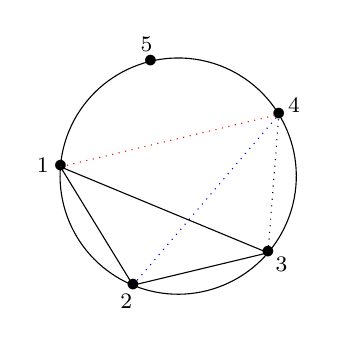
\begin{tikzpicture}[rotate=67.5,baseline=(current bounding box.east)]
	\begin{scope}
		\drawboundary{5}{1.5}
		\drawnumbersshift
		\drawchord{1}{4}{red, dotted}
		\drawchord{2}{4}{blue, dotted}
		\drawchord{3}{4}{dotted}
		\drawchord{1}{2}{}
		\drawchord{2}{3}{}
		\drawchord{3}{1}{}
	\end{scope}  \end{tikzpicture} 
 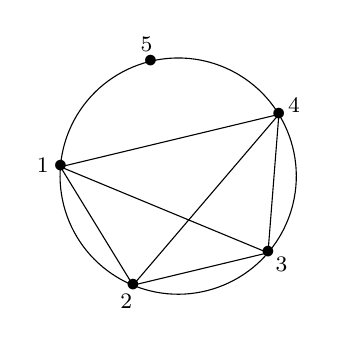
\begin{tikzpicture}[rotate=67.5,baseline=(current bounding box.east)]
	\begin{scope}
		\drawboundary{5}{1.5}
		\drawnumbersshift
		\drawchord{1}{4}{}
		\drawchord{2}{4}{}
		\drawchord{3}{4}{}
		\drawchord{1}{2}{}
		\drawchord{2}{3}{}
		\drawchord{3}{1}{}
	\end{scope}
\end{tikzpicture} \;.\eas
In the left diagram, $\sC = \{\{1, 2, 3\}, \{1, 4\}, \{1, 3\} \{1, 2\}\}$, while in the right diagarm $\sC = \{\{1, 2, 3, 4\}\}$. Thus both sets of minimal dependent sets (and thus the corresponding independence systems have the same underlying graph.
\end{eg}

\begin{lem}\label{res:matroidsimplex}
The graph $\cT$ defines a matroid if and only if for every pair of maximal complete subgraphs, $S, T$, if $x\in V(S) \cap V(T)$ then there is another maximal complete subgraph $U$ with $V(U) \subsetneq (V(S) \cup V(T)) \setminus 
\{x\}$. 
\end{lem} \sanote{fix this later when the correct graphical representation is chosen}
\begin{proof}
By Lemma \ref{res:graphtoindepsys}, the graph  $\cT$ gives rise to an independence system. Specifically, every maximal complete subgraph of $\cT$, $S \in \cS$ is a minimal dependent set of the corresponding independence set $\sI$.

An independence system gives rise to a matroid if and only if the minimal dependent sets satisfy the circuit condition, \eqref{eq:circuitcondition}, which is exactly the condition in the Lemma.
\end{proof}

Note that the graph $\cT$ need not be connected. We denote the connected components of $\cT$ as $X^i$. 

\begin{dfn}
	Let $M = (E, \sI)$ be a matroid. We write $\cT_M$ be the graph associated to the independence system, $\sI$.
\end{dfn}

In order to better understand the connection between the matriod structure of $M$ and the graph $\cT_M$, we work through how to identify other structures from the simplex set. The graph $\cT_M$ is better suited for working with circuits than the other equivalent definitions. However, for completeness, we show how to translate from one to another.

Recall that the basis set, $\cB_M$ of $M$ is the maximal set of independent sets in $[n]$ and $\cC_M$ the set of circuits. Furthermore, if $S \in \cC_M$, the complete subgraph $\cK(S)$ is a maximal complete subgraph of $\cT_M$. By construction, for $S \in \cC$, any proper subset of $S$ is independent. Since the elements of $\cB_M$ are both maximal and independent, a set $B \subseteq E$ is in $\cB_M$ if and only if the restriction of $\cT_M$ to $B$ does not contain any element of the from $\cK(S)$, for some $S \in \cC_M$ (by independence) and, for any $x \in [n] \setminus B$, $\cT$ restricted to $B \cup x$ contains a subgraph of the from $\cK(S)$, for some $S \in \cC_M$ (by maximality).

Given any subset $D \subseteq [n]$, we may define the closure of $D$, $\cl(D)$. By definition, for any $x \in [n] \setminus \cl(D)$, $\rk(\cl(D)) < \rk(\cl(D) \cup \{x\})$, and for any $x \in \cl(D)$, $\rk(D) = \rk(D \cup \{x\})$. Therefore, if there is an $S \in \cC$ such that $D \setminus S = \{x\}$, then, since $\rk(S \setminus x) = \rk(S)$, we know that $x \in \cl(D)$. Furthermore, for $x \in [n] \setminus D$, if $\rk(D \cup \{x\}) = \rk(D)$, we know that $x$ is an element of a minimal dependent set, $S$, with all but one element in $D$. Indeed if every $S \in \cC_M$ containing $x$ satisfied $|S \setminus D| >1$, then $\rk(D \cup \{x\}) = \rk(D) +1$. Therefore, define $\cC_D = \{S \in \cC_M | |S \setminus D| <1 \}$. Then \ba \cl(D) = D \bigcup_{S \in \cC_D} S \label{eq:graphicclosure}.\ea


If the set $\cl(D)$ can be written as a union of elements of $\cC_M$, we say it is a cyclic flat.

\subsection{Matroid containment and simplices} \sanote{Transfer maximal complete graph language here.}
The overall goal of this paper is to determine the set of postroids of the largest dimension that are contained in a given matroid. %We begin by showing how, given a simplex $\cT_M$, to derive different  simplex $\cT$ such that $\cT$ defines a matroid $M'$ contained in $M$. 
For independence systems, one system is considered larger than another by set containment: $\sI'$ is contained in $\sI$ if and only if $\sI' \subseteq \sI$, or, equivalently, for every $B' \in \sB'$, there is a $B \in \sB$ such that $B' \subseteq B$. This extends to the concept of matroid containment. However, for positroids, we add the additional constraint that the two positroid be of the same rank. In other words, if $M' = ([n], \cB_{M'})$ and $M = ([n], \cB_{M})$ are two positroids, $M'$ contained in $M$ if and only if $\cB_{M'} \subsetneq \cB_{M}$.

%More generally,  there are four possible changes to $\cT$ (with a set of top dimensional cells $\sC$) that can be made to transform it into $\cT'$ (with a set of top dimensional cells $\sC'$): one can replace a top dimensional cell $S \in \sC$ with a set of its faces $F_S$ such that no element of $F_S$ is a face of another (we call this restricting to faces of $S$); one can remove one of the top dimensional cells; one can add a new top dimensional cell; and one can replace a set of top dimensional cells $\sC \in \sC$ with a larger cell, $T$ such that each $S \in \sC$ is a face of $T$ (we call this extending $S$). Any simplex on a set of vertices can be changed to another simplex on the same set by a combination of the above four steps.

We begin by translating the containment condition for independence systems onto the set of minimal dependent sets. 

\begin{lem} \label{res:indepcontainment}
Let $\sC$ and $\sC'$ be two sets of minimally dependents subsets of a ground set $E$, with associated graphs $\cT$ and $\cT'$ and independence systems $\sI$ and $\sI'$ respectively. We have containment of independence systems, $\sI' \subseteq \sI$ if and only if, for every $C \in \sC$ there is a $C' \in \sC$ such that $C' \subseteq C$.
\end{lem}
\begin{proof}
The independence system $\sI' \subsetneq \sI$ if and only if there is the reverse containment of dependent sets: $\sI^c \supsetneq \sI'^c$. Therefore, if $C \in \sC$ it is a dependent set according to $\sI'$, but it may not be minimal. In otherwords, every minimal dependent set according to $\sI'$, i.e. ever element of $\sC'$ is contained in an element of $\sC$.
\end{proof}

In other words, if $\sC$ is represented by the graph  
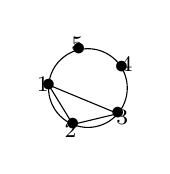
\begin{tikzpicture}[rotate=67.5,baseline=(current bounding box.east)]
	\begin{scope}
		\drawboundary{5}{.5}
		\drawnumbersshift
		\drawchord{1}{2}{}
		\drawchord{2}{3}{}
		\drawchord{3}{1}{}
	\end{scope}  \end{tikzpicture}, 
 then
  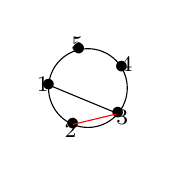
\begin{tikzpicture}[rotate=67.5,baseline=(current bounding box.east)]
	\begin{scope}
		\drawboundary{5}{.5}
		\drawnumbersshift
		\drawchord{2}{3}{red}
		\drawchord{3}{1}{}
	\end{scope}  \end{tikzpicture} and
  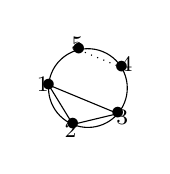
\begin{tikzpicture}[rotate=67.5,baseline=(current bounding box.east)]
	\begin{scope}
		\drawboundary{5}{.5}
		\drawnumbersshift
		\drawchord{5}{4}{dotted}
		\drawchord{1}{2}{}
		\drawchord{2}{3}{}
		\drawchord{3}{1}{}
	\end{scope}  \end{tikzpicture} 
 both define independence systems that are contained in that defined by $\sC$ but  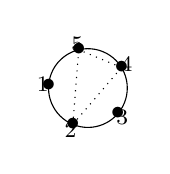
\begin{tikzpicture}[rotate=67.5,baseline=(current bounding box.east)]
	\begin{scope}
		\drawboundary{5}{.5}
		\drawnumbersshift
		\drawchord{4}{5}{dotted}
		\drawchord{2}{5}{dotted}
		\drawchord{2}{4}{dotted}
	\end{scope}  \end{tikzpicture}
or 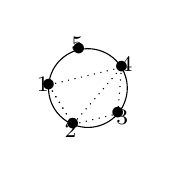
\begin{tikzpicture}[rotate=67.5,baseline=(current bounding box.east)]
	\begin{scope}
		\drawboundary{5}{.5}
		\drawnumbersshift
		\drawchord{1}{2}{dotted}
		\drawchord{1}{2}{dotted}
		\drawchord{2}{3}{dotted}
            \drawchord{1}{4}{dotted}
            \drawchord{2}{4}{dotted}
            \drawchord{3}{4}{dotted}
	\end{scope}  \end{tikzpicture}
do not.

We may talk about a largest independence system that is contained in another, as a pair of systems, $\sI$ and $\sI'$ such that $\sI' \subsetneq \sI$ but there does not exist another system $\sI''$ such that $\sI' \subsetneq \sI'' \subsetneq \sI$.

\begin{lem}
Let $\sC$ the set of minimal dependent sets of an independence system $\sI$ on the base set $E$. Let $\sB$ be the maximal independent sets of the independence system. Then $\sC'$ is the set of minimal dependent sets of a largest independence system contained in $\sI$ if and only if $\sC = \sC \cup B$, for some $B \in \sB$.
\end{lem}
\begin{proof}
Let $\sI'$ be an independence system that is one of the largest (under containment) strictly contained in $\sI$. Then $\sI' = \sI \setminus B$ for some $B \in \sB$. Otherwise, if $I \in \sI \setminus \sI'$ where $I$ is not a maximally independent set of $\sI$, then by downward closedness, there is a larger set $B \in \sB$, such that $\sI \subsetneq B$ and $B \not \in \sI'$. In other word, $\sI' \subsetneq \big(\sI \setminus B) \subsetneq \sI$. 

Since $\sI' = \sI \setminus B$, $B$ is a minimal dependent set in $\sI'$. I.e. $\sC' = \sC \cup B$.
\end{proof}

While there are many possible independence systems strictly contained in any given independence system, if there is an largest matroid contained in an independence system that is not a matroid. 

START HERE.

To do this, we establish some notation. Let $X \subset E$ be the set of elements contained in the intersection of two different elements of $\sC$: $X = \{ (x, C_1, C_2 )| a \in C_1 \cap C_2, \; C_1, C_2 \in \sC\}$. We construct the largest indepedence set contained in $\cI$ by the following algorithm.

\begin{alg}
    For $\sC$ a set of minimal dependent sets and $X$ the set of points in its intersections, we define another set of minimal dependent sets, $\sC'$ as follows:
\begin{enumerate}
    \item Let $X_\emptyset = \{(x, C_1, c_2) \in X | \forall C \in \sC , C \cap \big((C_1 \cup C_2) \setminus x\big) = \emptyset\}$ 
    \item Let $X_\subseteq = \{(x, C_1, c_2) \in X | \exists C \in \sC , C \subseteq \big((C_1 \cup C_2) \setminus x\big)\}$
    \item Let $X_\cap = X \setminus \big(X_\emptyset \cup X_\subsetneq$. 
    \end{enumerate}
That is, if $(x, C_1, c_2) \in X_\cap$ there is a $C \in \sC$ such that $C \cap \big((C_1 \cup C_2) \setminus x\big) \neq C, \emptyset$.

We build $\sC'$ elementwise on $X$. For all $(x, C_1, c_2) \in X_\subset$, $\sC$ does not change. For all $(x, C_1, c_2) \in X_\emptyset$, add the element add the set $\big((C_1 \cup C_2) \setminus x\big)$ to $\sC$. At the end of this step, $\sC' = \sc$ 
\end{alg}


For each $x \in X_\sC$, define a set of sets $C_x$ as $C_x = \{ C \in \sC | C \subseteq C_1 \cup C_2 \setminus a \}$ if there is an element of $\sC$ contained in the set $C_1 \cup C_2 \setminus a$. Set $C_x = \{C_1 \cup C_2 \setminus a \}$ if no element of $\sC$ intersects $C_1 \cup C_2 \setminus a$. \hlfix{Finally set $C_x = \{C \cap \big(C_1 \cup C_2 \setminus a \big), C \setminus \big(x, C_1, C_2 \big) | C \cap \big(C_1 \cup C_2 \setminus x \big) \neq \emptyset, C \}$.}{this is not right.}

\begin{lem}
    Let $\sI$ be an independence system on $E$ that does not define a matroid, with set of minimal dependence sets $\sC$. Then, the largest independence system that is both contained in $\sI$ and defines a matroid is defined by the set of minimal dependent sets $\sC' = \sC \cup_{x \in X_\sC} C_x$.
\end{lem}
\begin{proof}
    Since $\sI$ is an independence system that does not define a matroid, the associated set of minimal dependent sets $\sC$ does not satisfy the circuit condition, \eqref{eq:circuitcondition}. That is, there is some $x \in X_\sC$ such that there is not an element $C \in \sC$ such that $C \subseteq C_1 \cup C_2 \setminus a$. For this $x$, $C_x \not \subseteq \sC$. Therefore, $\sC'$ strictly contains $\sC$. Therefore, the associated independence set $\sI'$ is contained in $\sI$. 

    Furthermore, notice that by construction, $X_\sC \subsetneq X_{\sC'}$. If $x \in X_\sC$, each set $C_x$ contains at least one element that is contained in $C_1 \cup C_2 \setminus a$. Therefore, the set of sets $\sC'$ satisfies the circuit condition, i.e. defines a matroid. \sanote{fix para after fixing $C_x$} 
\end{proof}
\begin{comment}
Furthermore, we show that adding a top dimensional simiplex, or restricting to proper faces are suffienct moves to transition between any two simplices $\cT$ and $\cT'$ on $[n]$, where the the independent sets of $\cT'$ are strictly contained in the independent sets of $\cT$. 

\begin{prop} \label{res:containmentmoves}
Let $\cT$ and $\cT'$ two simplices, (with sets of top dimensional cells $\sC$ and $\sC'$ respectively) such that the independent set of $\cT'$ are strictly contained in the independent sets of $\cT$. Then  $\sC' = ((\sC \cup \{U\}) \setminus \{S\}) \cup \bigcup_{S \in \{S\}} F_S$, where $\{U\}$ is a set of top dimensional cells not in $\sC$, $\{S\} \subseteq \sC$ and $F_S$ a non-empty set of faces of $S$ that are top dimensional in $\sC'$. 
\end{prop}
\begin{proof}
 By hypothesis, there exists a set $I$ that is independent according to $\cT$ but not $\cT'$. Then $I$ contains the vertices of an element $U \i \sC'$ that is not in $\sC$: $U \not in \sC$. There are two possible cases: either $U$ is a face of some $S \in \sC$ or it is not.

In the first case, $U$ results from the restriction of some $S \in \sC$. That is, $U \in F_S$.

In the second case, there is not a $S \in \sC$ such that $U$ is a face of $S$. Therefore, since $U \not \in \sC$, it is a new top dimensional cell added to $\sC$. 
\end{proof} 

Putting these together, we get a condition on the simplices associated to a pair of matroids where one basis set it contained in the other. 

\begin{cor}Let $M$ and $M'$ be two matroids on $[n]$ with $\cB_M \supsetneq \cB_{M'}$. Then $\cT_{M'}$ (with top dimensional cells $\sC_{M'}$) is formed from $\cT_{M}$ (with top dimensional cells $\sC_{M}$) by either adding new cells or restricting existing cells to faces: \bas \sC_{M'} = ((\sC \cup \{U\}) \setminus \{S\}) \cup \bigcup_{S \in \{S\}} F_S \;.\eas
\end{cor}
\begin{proof}
This follows from Proposition \ref{res:containmentmoves}.
\end{proof}

In the following section, we provide some examples of these independence structures and their associated complettions.
\end{comment}

\subsubsection{Examples \label{sec:egs}} \sanote{work in progress}
We begin by giving  an example of a set that is not an independence system, names that does not satisfy the downward closed property, and demonstrate that this cannot be represented as a simplex.

\begin{eg}\label{eg:notasystem}
Consider the base set $[6]$, with $\sI = \{123, 124, 125, 345, 12, 13, 14, 15, 23, 24, 25, 45, 1, 2, 3, 4, 5, \emptyset \}$ Note that the set $\{3,4\}$ is in $\sI^c$, but that $\{3,4,5\}$ is in $\cI$. In otherwords, this is not a downward closed set of subsets. In this case, the set of minimal dependent sets is $\sC = \{6, 34, 1235, 1245\}$. All other elements of $\sI^c$ contain one of these elements. The set of maximal independent sets of $\sI$ is $\cB = \{123, 124, 125, 345\}$. Note that the set $\cB$ satisfies the basis exchange property and $\sC$ satisfies the circuit condition, however as $\sI$ is not downward closed, this is not a matroid. In particular, the set $\{3, 4, 5\}$ is a both a maximal independent set and contains a circuit, making it a dependent set. \sanote{needs a pict}
\end{eg}

On the other hand, note that \emph{any} matroid can be represented in this manner, and not just representable ones.

\begin{eg}
The Fano matroid is a matroid on $7$ points, with $7$ cyclic flats of rank $1$ each. This matroid is not representable. However, it does have an associated simplex. Namely, we may write the circuits of rank $2$  as $\{1, 2, 3\}, \{ 3, 4,5\}, \{5, 6,1\}, \{2, 4, 6\}, \{1, 7, 4\}, \{2, 7, 5\}, \{3, 7, 6\}$ and circuits of rank $3$ as $4$-tuples with exactly 2 pairs of vertices from two distinct circuits of rank $2$. Note that each element of $\sC$ is a cyclic flat, as each circuit intersects another at exactly one point.  
\end{eg}

Next we give a few examples of simplicial structures for 

\subsection{Matroid completions of simplices}

The above discussion allows one to define a matroid completion of a simplex, $\cT$. Given a simplex $\cT$ that does not satisfy Lemma \eqref{res:matroidsimplex}, i.e. that does not correspond to the independence system of a matroid, we wish to define a simplex $\overline{\cT}$ that does satisfy Lemma \eqref{res:matroidsimplex}, and such that the independent sets of $\overline{\cT}$ are a subset of the independent sets according to $\cT$.

\begin{dfn}
Given a simplex $\cT$, we define a matroid completion of $\cT$ to be $\overline{\cT}$ to be a simplex with the largest independence system contained in $\cT$ that is also the independence system of a matroid.
\end{dfn}

We note that the matroid completion of a simplex is not unique, and in the examples below, show instances where there are multiple different valid matroid completions. 

In the results below, we need the following nomencalture.

\begin{dfn} \label{dfn:matroidcompletion}
Let $\cT$ be a simplex on $[n]$. Let $A = \{ (x, S, T) | x \in S \cap T; \; S, T \in \sC\}$.  For each $a= (x, S, T) \in A$, let $\Sigma_a$ be the simplex on the vertices $(S_0 \cup T_0)\setminus x$. We define three sets of simplices associated to each $a$, $U_a$, $V_a$ and $W_a$ in three cases:
\begin{enumerate}
\item If there is a cell $W_a \in \sC$ such that $\Sigma_a$ is a face of $W_a$, we define $U_a = \Sigma_a$ and $V_a$ the simplex on the remaining vertices of $W_a$. 
\item If there is a cell $W_a \in \sC$ that is a face of $\Sigma_a$, we set $U_a := W_a$, $V_a$ is the empty simplex. 
\item Otherwise, there is no simplex on the vertices $(S_0 \cup T_0)\setminus x$, i.e. $W_a = \emptyset$, we set $U_a = \Sigma_a$ and $V_a$ is the empty simplex.
\end{enumerate}
Then the matroid completion of $\cT$ is given by \ba \overline{\cT} = \cT \bigcup_{a \in A} (U_a \cup V_a) \setminus \bigcup_{a \in A} W_a\;. \label{eq:matroidcompletion}\ea 
\end{dfn}

Note that in the first two cases of Definition \ref{dfn:matroidcompletion}, $\Sigma_a$ cannot be a top dimensional cell, i.e. an element of $\sC$. In the first case, this is because there is already an element $U \in \sC$ that contains it, and in the second case because there is an already an element $U \in \sC$ contained in it. In other words, Definition \ref{dfn:matroidcompletion} adds $\Sigma_a$ to $\sC$ if that is a valid top dimensional cell, does nothing if the vertices of $\Sigma_a$ already contain a top dimensional cell, and breaks a larger top dimensional cell $W_a$ containing $\Sigma_a$ into two simplices, $\Sigma_a$ and its complement.

\begin{prop}
The simplex $\overline{\cT}$ defines a matroid.
\end{prop}
\begin{proof}
	We check that the matroid completion, $\overline{\cT}$ satisfies the condition in Lemma \ref{res:matroidsimplex}. 
	
	First note that if $S, T \in \sC$ are two top dimensional simplices in different connected components of $\cT$, then $S_0 \cap T_0  =\emptyset$. Furthermore, $\cT$ has the same number of connected components as $\cT$. Therefore, we may restrict to the case where $\cT$ has one connected component. Furthermore, we may assume that $\sC$ has at least two elements. 
	
	Suppose $x \in S_0 \cap T_0$. Let $a = (x, S, T)$. By construction $U_a$ is top dimensional. Therefore, $\overline{\cT}$ defines a matroid.
\end{proof}

Note, the matroid completion of a simplex is not necessarily the only matroid structure with bases contained in the independence system of $\cT$. In Proposition \ref{res:completionbiggest}, we show that this is the largest matroid with compatible independence system. First we give an example of the multiple matroids with compatible independence systems. 

\begin{eg}
THIS NEEDS A PICTURE.

For $n \geq 4$, let $\cT$ be a simplex on $n$ with a $2$ simplex $S = \{1, 2, 4\}$ and another one $T = \{1, 2, 3\}$ and all its faces. This is not a matroidal, as there is not a simplex in $S_0 \cup T_0 \setminus 1$ or $S_0 \cup T_0 \setminus 2$. 

If we add the cell $U = \{3, 4\}$ and all its faces to $\cT$, the new simplex $\cT' = \cT \cup U$ is matroidal. However, it is not the matroid completion. 

According to Definition \ref{dfn:matroidcompletion}, $\overline{\cT}$ has the two additional $2$ simplices (and all the faces) of $V = \{1, 3,4 \}$ and $W  = \{2, 3,4 \}$. 

Note that the matroid associated to $\overline{\cT}$ is larger than that associated to $\cT'$. Namely, in $\overline{\cT}$ the vertices $\{3, 4\}$ are independent, but not in $\cT'$.
\end{eg}

\begin{prop}\label{res:completionbiggest}
The simplex $\overline{\cT}$ is the largest matroid with independent sets contained in the sets independent according to $\cT$.
\end{prop}
\begin{proof}
NO IDEA
\end{proof}

\subsection{Positroids as simplices}

In this section, given a matroidal simplex $\cT_M$, we give a condition for when $M$ is a positroid. We prove this by using the fact that the matroid $M = ([n], \cB)$ is a positroid if and only if $\cI_\cB = \cB$ as shown in equation \eqref{eq:I_B}. If $M$ is not a positroid, then $\cI_\cB \supsetneq \cB$. 

We begin by introducing some notation.

\begin{dfn}
Let $F$ and $G$ be two flats of a matroid on $[n]$. We may write each as a disjoint union of cyclic intervals in $[n]$: $F = F_1\sqcup \ldots F_d$ and $G = G_1\sqcup \ldots G_{d'}$, with $F_i$ and $G_i$ corresponding to two maximal cyclic subsets of $F$ and $G$ respectively. Similarly the complements $F^c$ and $G^c$ can be writen as a disjoint set of cyclic intervals: $F^c = F^c_1\sqcup \ldots F^c_d$ and $G^c = G^c_1\sqcup \ldots G^c_{d'}$, with the vertices of $F^c_i$ between the vertices of $F_{i}$ and $F_{i+1}$. We say that two flats, $F$ and $G$ are crossing if $F$ intersects two intervals in the complement of $G$:\bas \exists i \neq j  \textrm{ such that } F\cap G^c_{i} \neq \emptyset \textrm{ and } F\cap G^c_{i} \neq \emptyset. \eas
\end{dfn}

\begin{thm}
Let $\cT$ be a simplex that captures the independence systems of a matroid $M$ with $\sC$ the set of top dimensional cells. For $S \in \sC$, with vertices $S_0$, let $\cl(S)$ be the closure of the set $S_0$. Let $[a_S, b_S] \subseteq [n]$ be a cyclic interval containing $\cl(S)$ with $a_S, b_S \in \cl(S)$. Then $M$ is not a positroid if and only if there is an element $T \in \sC$, such that the closure $\cl(T)$ crosses $\cl(S)$.
\end{thm}
\begin{proof}
For a matroid $M = ([n], \cB)$, we show that $\cB = \cI_\cB$ if and only if for every $S, T \in \cl(S)$ and the closure $\cl(T)$ intersects only one cyclic interval in the complement of $\cl(S)$.

Let $M$ be a matroid of rank $k$. Suppose we are in the situation where no flats of the form $\cl(\sC)$ cross. Write $F = \cl(S)$. Then the closure of any cyclic interval in the complement of $F$ is contained in the $\cl(\sC)$ and said interval: \ba \cl(F_j^c) \subseteq F_{j} \cup F^c_{j} \cup F_{j+1}\;. \label{eq:noncrossingclosurecond}\ea Moreover, $|I_i \cap F^c_j| = r$ for every $I_i \in \cI$. \sanote{make this a lemma, not quite right... discuss}.

Let $B$ be a dependent set of size $k$: $|B| = k$. Since $B$ is a dependent set, it contains a circuit, $S$. By abuse of notation, let $S \in \sC$ be the corresponding top dimensional simplex with $F = \cl[S]$. We know that for any $i \in [n]$ the Grassmann necklace element $I_i$ has exactly $\rk(S)$ elements in $F$. However, $S \subseteq B$, and therefore $B$ has at least $\rk(S) + 1 $ elements in $F$. Since both $B$ and $I_i$ have $k$ elements, this means that there is some cyclic interval in $F^c$, call it $F^c_j$, where $I_i$ has more elements than $B$: $|I_i \cap F^c_j| > |B \cap F^c_j|$. For ease of reference, let $|I_i \cap F^c_j| = r$ and $|B \cap F^c_j|=s$, with $r > s$. Furthermore, by equation \eqref{eq:noncrossingclosurecond}, this interval is the same for any index $i$. There is no way for $I_i$ to contain any elements in $\cl(F_j^c)$ other than in the cyclic interval $F_{j} \cup F^c_{j} \cup F_{j+1}$.

Let $a = F_{j+1}^{(1)}$ be the first element in $F$ after the cyclic interval $F_j^c$. Then, in the $<_a$ order, the element $B^{(k-s)}$ is in $F_{j}$ while $I_a^{(k-s)}$ is in $F^c_{j}$. I.e, $B^{(k-s)} <_a I_a^{(k-s)}$. Therefore, $I_a \not \preceq_a B$. Since we can find such an element $a$ for any dependent set $B$, we see that if $B$ is a dependent set in $M$, then $B \not \in \cI_\cB$. Therefore $\cI_\cB = \cB$, and $M$ is a positroid.
 
Now suppose we are in the setting where the closures of two circuits may cross. Let $F = \cl(S)$ and $G = \cl(T)$ be the two crossing flats in question. Then we may write $F = F_1 \sqcup \ldots \sqcup F_d$ and $G = G_1 \sqcup \ldots \ldots G_{d'}$. Fix a vertex $i$ not in $F$: $i \in F^c$. Without loss of generality, assume that $i \in F^c_d$. Let $x \in I_i$ be the first element of $I_i$ (in the $<_i$ order) that is in $G$. Furthermore, notice that since $I_i \cap F$ has fewer than $\rk(F)$ elements, then $F_d$ has some elements not in $I_i$: $F_d \setminus I_i\neq \emptyset$. Let $y$ be any such element, $y \in F_d \setminus I_i$. Define $B = (I_i \setminus x) \cup y$. This set $B$ has $k$ elements, $\rk(F)+1$ are in $F$, making it a dependent set, and ensuring that $B \not \in \cB$.

Next, we show that $B \in \cI_\cB$, making $B \subsetneq \cI_\cB$, and $M$ not a positroid. We check that for every $a \in [n]$, $I_a \preceq_a B$. Recall that for any $a \in [n]$, since both $I_i$ and $I_a \in \cI$, we have that $I_a \preceq_a I_i$, and specifically, $I_a^{(l)} \leq_a I_i^{(l)}= x$. Therefore, if $x <_a y$ (i.e. $a \in [y+1, x]$), then $I_a <_a B$. If $y <_a x$ (i.e. $a \in [x+1, y]$), there are two cases to consider. Either $G\cap I_a = G \cap I_i$ or there exists an element $z \in G \cap I_a \setminus I_i$. These are the only two cases since every Grassmann necklace element has $\rk(G)$ elements in $G$. 

If $G\cap I_a = G \cap I_i$, and $I_a \preceq_a I_i$, we know that every element of $I_i\cap G$ occurs later in the series $I_i$ (according to the $<_a$) order than in the series $I_a$. Therefore, $B$, which is formed by removing $x \in I_i \cap G$ from $I_i$ and replacing it with an element $y$ with precedes $x$ in the $<_a$ order ($a <_a y <_a x$) means that $I_a \preceq_a B$.

If there exists a $z \in G \cap I_a \setminus I_i$ and $a <_a y <_a x$, then write $I_a^{(r)} = z$ and $I_i^{(l)} = i$. Since $a \in [x+1, y]$ we have that $r < l$. Since $B = (I_i \setminus x) \cup y$ we know that $z \not \in B$. Therefore, since $I_a \preceq_a I_i$, we have that $I_z \preceq_a B$.

\end{proof}

Note that we don't claim that a matroid is a positroid if and only if no cyclic flats cross. That is not true. See Example \ref{eg:???}. We claim that a matroid is a positroid if and only if the closures of the circuits do not cross. \sanote{write an example here}

\bibliographystyle{abbrv}
\bibliography{Bibliography}


\end{document}